\documentclass[spanish,12pt,a4paper,titlepage]{report}
\usepackage[latin1]{inputenc}
\usepackage{graphicx}
\usepackage{subfig}
\usepackage{float}
\usepackage{wrapfig}
\usepackage{multirow}
\usepackage{caption}
\usepackage{babel}
\usepackage[dvips]{hyperref}
\usepackage{amssymb}
\usepackage{listings}
\usepackage{epsfig}
\usepackage{amsmath}
\usepackage{array}
\usepackage[table]{xcolor}
%\usepackage{multirow}
%\usepackage[Sonny]{fncychap}
%\usepackage[Glenn]{fncychap}
\usepackage[Conny]{fncychap}
%\usepackage[Rejne]{fncychap}
%\usepackage[Bjarne]{fncychap}

\setlength{\topmargin}{-1.5cm}
\setlength{\textheight}{25cm}
\setlength{\oddsidemargin}{0.3cm} 
\setlength{\textwidth}{15cm}
\setlength{\columnsep}{0cm}

\begin{document}

\chapter{Comparacion de Hardware}
%\thispagestyle{plain}
%\pagestyle{fancy}


La eleccin del Hardware significa una parte muy importante del Proyecto, ya que las decisiones tomadas condicionan el resto del mismo. Una mala eleccin de alguno de los componentes puede resultar en complicaciones no previstas a la hora de la ejecucin, causando contratiempos inesperados y trabajo excesivo. Es necesario entonces para evitar dichos problemas el estudio detallado de cada uno de los componentes a utilizar, comparando caractersticas, rendimientos y utilidades. \\
Elegir adecuadamente el Hardware necesario agiliza las etapas siguientes de todo el Proyecto. Resulta fundamental la toma de buenas decisiones, las cuales deben estar basadas en un previo estudio de cada etapa del proyecto, sus requerimientos, un estudio comparativo de las posibles soluciones y el conocimiento cabal de los componentes a utilizar.\\

\section{Eleccin de plataforma Cuadricpteros}
\vspace*{15pt}

A la hora de la planificacin del Proyecto se plantean dos opciones que se diferencian bsicamente en el punto de partida. Ambas tienen como objetivo principal disear e integrar un sistema de control que permita al Cuadricptero mantener un vuelo autnomo, pero una de ellas consta adems del en  el diseo y el armado del mismo. \\Esta ltima incluye desafos de ingeniera mecnica, conocimientos de resistencia, flexibilidad y peso de materiales, as como tambin diversas complicaciones a la hora de fabricar y armar las partes. \\ Teniendo en cuenta que se trata de un proyecto con tiempo acotado y su objetivo se centra en el control del vehculo, la necesidad de partir de con un hardware ya construido resulta imperiosa. Por ello se realiza un estudio sobre las opciones que el mercado ofrece en esta materia. Desafortunadamente las opciones no son muy numerosas, disponiendo de Cuadricpteros comerciales controlados a control remoto. Todos ellos incluyen un pequeo sistema de control integrado de los cuales no es posible obtener informacin ya que se trata de software privativo. Las opciones que el mercado ofrece son: 
\begin{itemize}
	\item Gaui 330X
	\item XAircraft X650
	\item Turbo Ace X720
\end{itemize}
Se procede a la comparacin de los equipos mencionados y se analizan algunos aspectos fundamentales y crticos, como puede ser por ejemplo el peso del dispositivo y la carga til que puede soportar.


\subsubsection*{Motor}
Al estudiar las posibilidades nos encontramos con que en todos los casos los motores se controlan con modulacin por ancho de pulsos, de ahora en ms \textbf{PWM} por sus siglas en ingls, tcnica en la cual se modifica el ciclo de trabajo de una seal peridica para controlar la cantidad de energa que se entrega a una carga.\\

	En la tabla \ref{tab:motor} se muestran las caractersticas de los motores de los 3 Cuadricpteros considerados.\\

\begin{table}[H]
\begin{tabular}{p{40pt}|p{80pt}|p{130pt}|p{130pt}|} 
\cline{2-4}
& \cellcolor[gray]{0.8} \textbf{GAUI 330X} 
& \cellcolor[gray]{0.8} \textbf{XAircraft X650} 
& \cellcolor[gray]{0.8} \textbf{Turbo Ace X720} \\ \cline{2-4} \hline
\multicolumn{1}{|p{40pt}|}{\cellcolor[gray]{0.8}\textbf{Motor}} 
& Hlices de 8 pulgadas, 4 motores brushless con 4 ESCs de 10A 
& Hlices de 12 pulgadas, 4 motores brushless con 4 ESCs de 10A. Las hlices impulsadas por el motor tienen una eficiencia de 9g/W bajo carga nominal. 
& Hlices de 12 pulgadas, 4 motores brushless con 4 ESCs de 10A. Las hlices impulsadas por el motor tienen una eficiencia de 12g/W bajo carga nominal.\\ \hline
\end{tabular} 
\caption{Comparacin motores}
\label{tab:motor}
\end{table}

	Los motores \emph{Brushless} son motores elctricos alimentados con corriente continua. Tienen un sistema de conmutacin elctrico y presentan relaciones lineales entre \emph{Corriente} y \emph{Torque} y entre \emph{Frecuencia} y \emph{velocidad}. Son comnmente utilizados en vehculos radio-controlados por su gran eficiencia, potencia, durabilidad y su bajo peso en comparacin con los tradicionales motores \emph{Brushed}. Sin embargo, los motores de CC \emph{Brushless} son mucho ms complicados de controlar, ya que la fase vara con la rotacin del motor. Para controlarlos se utilizan unos dispositivos llamados \emph{Controladores elctricos de velocidad}, o \textbf{ESCs}. Comnmente los ESCs se clasifican segn su corriente mxima, por ejemplo 10 ampres o 10A.\\

	Como se puede ver en la tabla \ref{tab:motor}, todos los dispositivos utilizan motores similares y la nica diferencia radica en que la eficiencia de los motores del \emph{Turbo Ace X720} es mayor.

\subsubsection*{Tiempo de vuelo}

	El tiempo de vuelo puede resultar crtico segn la aplicacin considerada. En la tabla \ref{tab:tiempo} se muestran los datos que se obtuvieron para los 3 Cuadricpteros considerados.

\begin{table}[H]
\begin{tabular}{p{40pt}|p{80pt}|p{130pt}|p{130pt}|} 
\cline{2-4}
& \cellcolor[gray]{0.8} \textbf{GAUI 330X} 
& \cellcolor[gray]{0.8} \textbf{XAircraft X650} 
& \cellcolor[gray]{0.8} \textbf{Turbo Ace X720} \\ \cline{2-4} \hline
\multicolumn{1}{|p{40pt}|}{\cellcolor[gray]{0.8}\textbf{Tiempo de vuelo}} 
& Con batera de $2200 mAh$ vuela entre 7 y 20 minutos & Vuela 12 minutos con batera de $2200mAh$ y carga menor a $1.5kg$ & Con batera de $2200mAh$ vuela 15 minutos a carga nominal y puede llegar a la media hora de vuelo con una batera de $10.000mAh$ \\ \hline
\end{tabular}
\caption{Comparacin Tiempo de vuelo}
\label{tab:tiempo}
\end{table}

	Como se puede apreciar los tiempos de vuelo son similares en los 3 dspositivos, por lo que no ser un factor determinante a la hora de tomar la decisin.\\

	Un factor determinante en el tiempo de vuelo es la batera a utilizar. Deben considerarse 2 aspectos importantes: la capacidad de la batera y su peso. Si bien una batera con mayor capacidad permitir mayor autonoma de vuelo, es claro que su peso tambin aumentar, lo cual a su vez, causar un mayor consumo. Los 3 Cuadricpteros en consideracin incluyen una batera de 3 celdas de Litio de $2200 \, mAh$.

\subsubsection*{Peso}

	La carga til que el dispositivo pueda soportar juega un papel fundamental. Vale recordar que adems de toda la instrumentacin que incluye el Cuadricptero, se incorporar un Microprocesador, una batera independiente para su alimentacin, un girscopo, un acelermetro, un GPS y alguna interfaz para la comunicacin. A su vez es interesante conservar la posibilidad de integrar una cmara fotogrfica convencional ya que puede ser de gran utilidad para numerosas aplicaciones. La fuerza que los motores pueden realizar es acotada, por lo que el peso del dispositivo influye directamente en la carga til del mismo.

\begin{table}[H]
\begin{tabular}{p{40pt}|p{70pt}|p{160pt}|p{110pt}|} 
\cline{2-4}
& \cellcolor[gray]{0.8} \textbf{GAUI 330X} 
& \cellcolor[gray]{0.8} \textbf{XAircraft X650} 
& \cellcolor[gray]{0.8} \textbf{Turbo Ace X720} \\ \cline{2-4} \hline
\multicolumn{1}{|p{40pt}|}{\cellcolor[gray]{0.8}\textbf{Peso}} 
& $700g$ & Versin de fibra de vidrio: $1100g$. Versin de fibra de carbono: $950g$. & $990g$ \\ \hline
\multicolumn{1}{|p{40pt}|}{\cellcolor[gray]{0.8}\textbf{Carga til}} 
& $500g$ & Versin de fibra de vidrio: $700g$. Versin de fibra de carbono: $850g$. & $1300 g$ \\ 
\hline 
\end{tabular}
\caption{Comparacin peso y carga til}
\label{tab:peso}
\end{table}

Como se puede ver en la tabla \ref{tab:peso}, no cabe duda que el dispositivo que puede cargar con ms peso es el \emph{Turbo Ace X720}, lo cual constituye una ventaja considerable de este dispositivo frente a los otros.

\subsubsection*{Instrumentacin}

	Toda la instrumentacin que los dispositivos brindan est originalmente destinada al manejo mediante el control remoto. Todos ellos incluyen un acelermetro y un girscopo de 3 ejes y traen algn sistema de estabilizacin incluido de modo de facilitar su control. \\

	Como ya se mencion, se aadir al Cuadricptero la instrumentacin necesaria para su control automtico, por lo cual la instrumentacin incluida en el dispositivo carece de gran importancia. Sin embargo, resulta interesante conservar la posibilidad de controlarlo mediante el control remoto, ya que puede ser til tanto en determinadas aplicaciones, como para evitar eventualidades en las primeras pruebas donde se testean los algoritmos de control desarrollados. El algoritmo de control deber poder alternar entre estos dos modos de vuelo dndole prioridad al control remoto, de modo de conservar la integridad fsica del dispositivo ante fallas en los algoritmos de control.

\begin{table}[H]
\begin{tabular}{p{40pt}|p{85pt}|p{125pt}|p{130pt}|} 
\cline{2-4}
& \cellcolor[gray]{0.8} \textbf{GAUI 330X} 
& \cellcolor[gray]{0.8} \textbf{XAircraft X650} 
& \cellcolor[gray]{0.8} \textbf{Turbo Ace X720} \\ \cline{2-4} \hline
\multicolumn{1}{|p{40pt}|}{\cellcolor[gray]{0.8}\textbf{Instru- mentacin}} 
& Sistema de estabilizacin integrado \emph{GU344}: incluye girscopo de 3 ejes y acelermetro. & Girscopo de 3 ejes y acelermetro. Puede usar hasta 13 sensores para chequiar actitud de vuelo, altitud, direccin, posicin, temperatura, consumo energtico, etc. & Girscopo y acelermetro de 3 ejes integrados. Se vende por separado el mdulo GPS que incluye barmetro como medidor de altitud y el comps electrnico.\\ 
\hline 
\end{tabular}
\caption{Comparacin instrumentacin}
\label{tab:instrumentacion}
\end{table}

	En la tabla \ref{tab:instrumentacion} se muestra un resumen de la instrumentacin incluida en cada Cuadricpetro. 

\subsubsection*{Control}

	El control mediante el mando remoto requiere de cierta prctica y habilidad para ejecutarlo de buena forma, por lo cual todos los algoritmos de control integrados que el dispositivo incluya significarn una interesante ventaja. Por otro lado se debe tener en cuenta que el control remoto se utilizar en reducidos casos, siendo el control automtico el verdadero inters del proyecto. Es importante tener en cuenta que dichos algoritmos encarecen el precio del dispositivo y no sern utilizados con mucha frecuencia.

\begin{table}[H]
\begin{tabular}{p{40pt}|p{70pt}|p{160pt}|p{110pt}|} 
\cline{2-4}
& \cellcolor[gray]{0.8} \textbf{GAUI 330X} 
& \cellcolor[gray]{0.8} \textbf{XAircraft X650} 
& \cellcolor[gray]{0.8} \textbf{Turbo Ace X720} \\ \cline{2-4} \hline
\multicolumn{1}{|p{40pt}|}{\cellcolor[gray]{0.8}\textbf{Control}} 
& - & Software de configuracin incluido. Dispositivo de control de 4 velocidades diseado todo en 1. Soporta protocolos $Ultra$ $PWM$ y control de frecuencia hasta $500Hz$. Posee algoritmos de control de vuelo incorporados que hacen q sea mas fcil volarlo & Nivelacin automtica con control de altitud \\ 
\hline 
\end{tabular}
\caption{Comparacin control}
\label{tab:control}
\end{table}

	Si bien el \emph{XAircraft X650} es el que tiene ms algoritmos de control implementados que facilitan su mando, se considera que el dispositivo que se adeca ms a nuestras necesidades es el \emph{Turbo Ace X720}. Tiene un pequeo sistema de estabilizacin que ayuda a la hora de su control, pero no incluye demasiado software ni hardware que no ser utilizado y encarecen al producto, como el \emph{XAircraft X650}.

\subsubsection*{Dimensiones}

	Las dimensiones de los 3 Cuadricpteros considerados se pueden apreciar en la tabla \ref{tab:dimensiones}.

\begin{table}[H]
\begin{tabular}{p{40pt}|p{80pt}|p{130pt}|p{130pt}|} 
\cline{2-4}
& \cellcolor[gray]{0.8} \textbf{GAUI 330X} 
& \cellcolor[gray]{0.8} \textbf{XAircraft X650} 
& \cellcolor[gray]{0.8} \textbf{Turbo Ace X720} \\ \cline{2-4} \hline
\multicolumn{1}{|p{40pt}|}{\cellcolor[gray]{0.8}\textbf{Dimen- siones}} 
& 33 cm entre ejes diagonalmente opuestos & 61.5 cm entre ejes diagonalmente opuestos & 61.5 cm entre ejes diagonalmente opuestos \\ 
\hline 
\end{tabular}
\caption{Comparacin dimensiones}
\label{tab:dimensiones}
\end{table}

	Como se puede ver el \emph{GAUI} es el ms pequeo, mientras que los otros dos tienen el mismo tamao aproximadamente

	En la figura \ref{fig:cuadricopteros} se pueden apreciar fotografas de los 3 equipos considerados.

\begin{figure} [h!]
  \centering
  \subfloat[GAUI 330X]{\label{fig:gaui}
  		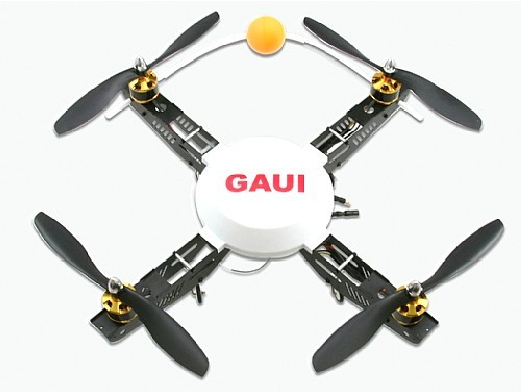
\includegraphics[width=0.3\textwidth]
  			{./pics_comparacion_hardware/gaui.png}}
  \subfloat[XAircraft X650]{\label{fig:aircraft} 
  		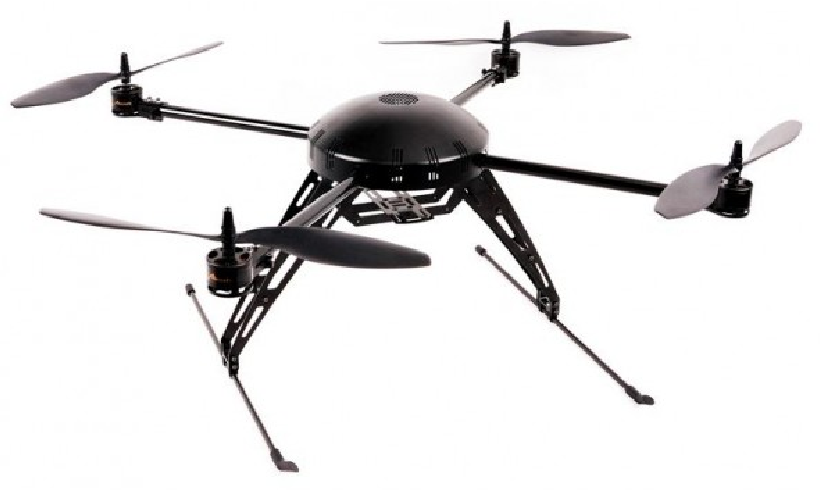
\includegraphics[width=0.36\textwidth]
  			{./pics_comparacion_hardware/aircraft.png}}
  \subfloat[Turbo Ace X720]{\label{fig:turboace} 
  		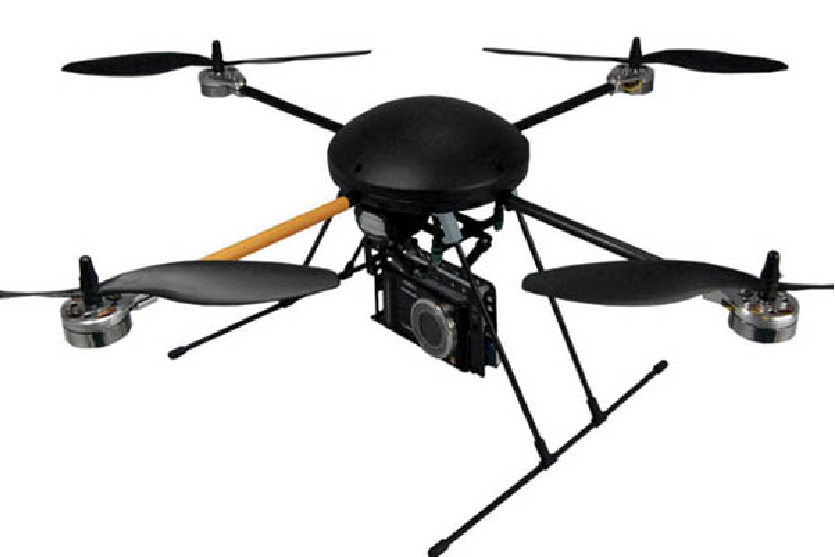
\includegraphics[width=0.32\textwidth]
  			{./pics_comparacion_hardware/turboace.png}}
  \caption{Fotos de las posibles plataformas a utilizar}
  \label{fig:cuadricopteros}
\end{figure}

\subsection{Definicin de la plataforma - Cuadricpetro}

\begin{itemize}
	\item El \emph{Turbo Ace X720} tiene hlices de 12 pulgadas y el grupo hlice motor proporciona una eficiencia de $12\,g/W$, superando a los otros dos Cuadricpteros considerados.
	\item La carga til que puede trasportar el \emph{Turbo Ace X720} es la mayor de todos los considerados
	\item El \emph{Turbo Ace X720} trae un sistema de nivelacin automtica y estabilizacin que resultar til al momento de controlarlo con el mando remoto. Adems no incluye excesivas utilidades para este mando que no sern utilizadas y contribuyen a encarecer el precio.
\end{itemize}

	Por todas las razones expuestas anteriormente y los anlisis comparativos realizados se tiene que la opcin que mejor se adeca a nuestro proyecto es el \textbf{Turbo Ace X720}. 

\newpage
\section{Inteligencia}
\vspace*{15pt}

Adems de la plataforma fsica, deben seleccionarse componentes electrnicos capaces de procesar la informacin proveniente de los sensores, computar y ejecutar los algoritmos de control y generar las seales necesarias para transmitir las instrucciones a los motores.\\
\\
Ser necesario, entonces, seleccionar uno (o varios) componentes capaces de desarrollar las tareas mencionadas. Para ello, el sistema elegido deber contar con:

\begin{itemize}
\item Un microprocesador con suficiente poder de computo
\item Un sistema de entradas y salidas que permita interactuar con la instrumentacin y con el sistema de control de motores
\item Un sistema de memoria no volil que permita mantener cargado el programa de control
\item Elementos de comunicacin para establecer conexin con un PC
\item Un sistema de potencia que brinde energa al sistema con una autonoma suficiente
\end{itemize}

Dado que el sistema utilizar motores brushless, es necesario contar con un sistema capaz de generar seales PWM, ya sea mediante software, hardware o ambas, para controlar los motores.\\
\\
Tambin ser necesario que el sistema seleccionado tenga una interfaz UART que permita la comunicacin con los sensores involucrados.\\
\\
Es evidente que la eleccin de la inteligencia no puede realizarse en forma independiente, sino que estar fuertemente condicionada por la eleccin del resto de la arquitectura del sistema final. Por ello, las decisiones tomadas sern afectadas considerablemente por las caractersticas del resto de los componentes del sistema.\\
\\
%Micro. decir pa q lo usamos, q tiene q hacer. payar
Teniendo en cuenta las restricciones anteriores, se seleccionaron varias arquitecturas posibles en una primera etapa. Se realizo un primer estudio de las diversas posibilidades ofrecidas, manejndose varias opciones.\\
\\
Varias de ellas fueron descartadas por no cumplir todos los requisitos arriba mencionados. De la opciones que s verificaban dichos requisitos fueron descartadas aquellas que implicaban ms de un componente, optndose por considerar las opciones que fueran capaces de proveer todas las opciones arriba mencionadas integradas en una nica placa.\\
\\
Una vez realizado un primer anlisis de las vastas posibilidades disponibles en el mercado se pre-seleccionaron las siguientes opciones:

\begin{enumerate}
\item Beagleboard XM

\item Gumstix Overo Fire
\end{enumerate}
A continuacin se desarrollaran y compararn las caractersticas fundamentales de ambas opciones, permitiendo as la seleccin de alguno de ellos en virtud de los requisitos del sistema que se desea implementar. 

\subsection*{Procesadores: CPU y DSP}
Es claro que el procesador es un componente determinante, pues ser el encargado de computar completamente los algoritmos de control. Tambin se encargar de manejar parte de la comunicacin con la instrumentacin y elementos de control. Finalmente, deber ser capaz de manejar informacin proveniente de los canales de comunicacin establecidos con un PC.

\begin{table}[H]
\begin{tabular}{p{130pt}|p{130pt}|p{130pt}|} 
\cline{2-3}
& \cellcolor[gray]{0.8} \textbf{Beagleboard XM} 
& \cellcolor[gray]{0.8} \textbf{Gumstix Overo Fire} \\ \cline{1-3} \hline
\multicolumn{1}{|p{130pt}|}{\cellcolor[gray]{0.8}\textbf{CPU}} 
&ARM Cortex A8 1Ghz,  256KB L2 cache, 1200 MIPS &ARM Cortex A8 720Mhz, 256KB L2 cache, 1200 MIPS \\ 
\hline 
\multicolumn{1}{|p{130pt}|}{\cellcolor[gray]{0.8}\textbf{DSP}} 
&TMS320C64x+, 800Mhz &TMS320C64x+, 520Mhz\\
\hline
\end{tabular}
\caption{Procesadores}
\label{tab:procesadores}
\end{table}

Resulta evidente que ambas opciones presentan el mismo procesador, con la salvedad que ambos procesadores de la Beagleboard presentan una mayor frecuencia de reloj. 

\subsection*{Memoria}

La memoria disponible en el sistema (tanto esttica como voltil) resulta de vital importancia, pues ser all que se guardar la informacin del programa de control, configuraciones, etc. Adicionalmente, es necesario contar con suficiente memoria voltil a la hora de procesar datos y ejecutar los algoritmos de control.\\

\begin{table}[H]
\begin{tabular}{p{130pt}|p{130pt}|p{130pt}|} 
\cline{2-3}
& \cellcolor[gray]{0.8} \textbf{Beagleboard XM} 
& \cellcolor[gray]{0.8} \textbf{Gumstix Overo Fire} \\ \cline{1-3} \hline
\multicolumn{1}{|p{130pt}|}{\cellcolor[gray]{0.8}\textbf{Voltil(RAM)}} 
&512Mb & 256Mb\\ 
\hline 
\multicolumn{1}{|p{130pt}|}{\cellcolor[gray]{0.8}\textbf{Esttica}} 
&Sin memoria interna.  Soporta microSD de hasta 4Gb  &256Mb de memoria interna\\
\hline
\end{tabular}
\caption{Memoria}
\label{tab:memoria}
\end{table}

La superioridad de la Beagleboard en cuanto a memoria resulta evidente a partir del anlisis anterior.

\subsection*{Dimensiones y peso}

Si bien no resulta una caracetrstica determinante, es conveniente que las dimensiones y peso de la placa elegida sean lo menores posibles, de forma de no ocupar gran parte de la carga til del cuadricptero con electrnica asociada a la inteligencia implementada.\\

\begin{table}[H]
\begin{tabular}{p{130pt}|p{130pt}|p{130pt}|} 
\cline{2-3}
& \cellcolor[gray]{0.8} \textbf{Beagleboard XM} 
& \cellcolor[gray]{0.8} \textbf{Gumstix Overo Fire} \\ \cline{1-3} \hline
\multicolumn{1}{|p{130pt}|}{\cellcolor[gray]{0.8}\textbf{Dimensiones}} 
&85.09x87.63mm &17x58mm\\ 
\hline 
\multicolumn{1}{|p{130pt}|}{\cellcolor[gray]{0.8}\textbf{Peso}} 
&36g &5.6g\\
\hline
\end{tabular}
\caption{Memoria}
\label{tab:memoria}
\end{table}
En cuanto a dimiensiones y peso, la placa Gumstix Overo Fire parece ser ms adecuada.

\subsection*{Programacin y Sistema Operativo}

Es importante tener en cuenta como ser realizada la programacin de los sistemas considerados (dnde se almacena el programa, hardware necesario para la programacin, etc.) En particular, es conveniente poder contar con algn sistema operativo que facilite la tareas de programacin, testeo y debugging.

\begin{table}[H]
\begin{tabular}{p{130pt}|p{130pt}|p{130pt}|} 
\cline{2-3}
& \cellcolor[gray]{0.8} \textbf{Beagleboard XM} 
& \cellcolor[gray]{0.8} \textbf{Gumstix Overo Fire} \\ \cline{1-3} \hline
\multicolumn{1}{|p{130pt}|}{\cellcolor[gray]{0.8}\textbf{Sistema Operativo}} 
&Booteable desde microSD &Booteable desde microSD\\ 
\hline 
\multicolumn{1}{|p{130pt}|}{\cellcolor[gray]{0.8}\textbf{Programacin}} 
&A travs de SO. Puerto JTAG de 14 pines &A travs de SO\\
\hline
\end{tabular}
\caption{Memoria}
\label{tab:memoria}
\end{table}

Es claro que la placa Beagleboard parece ser mejor en cuanto a sus prestaciones de programacin.

\subsection*{Alimentacin y Energa}

La forma en que la placa elegida es alimentada, as como el grado de autonoma que pueda lograrse con la misma deben ser tenidos en cuenta.\\
Lograr un nivel de autonoma lo suficientemente grande permitir que el sistema se mantenga en vuelo durante un tiempo mayor. Idealmente, la autonoma de la alimentacin de la inteligencia no debera ser el factor determinante del tiempo de vuelo del dispositivo.

\begin{table}[H]
\begin{tabular}{p{130pt}|p{130pt}|p{130pt}|} 
\cline{2-3}
& \cellcolor[gray]{0.8} \textbf{Beagleboard XM} 
& \cellcolor[gray]{0.8} \textbf{Gumstix Overo Fire} \\ \cline{1-3} \hline
\multicolumn{1}{|p{130pt}|}{\cellcolor[gray]{0.8}\textbf{Alimentacin}} 
& BeagleJuice. Sistema de alimentacin diseado especificamente para la Beagleboard. (Dimensiones idnticas a la misma. Conector estndar para BeagleBoard).
& Alimentado desde una Daughter board: Zippy Flightmax 2200mAh 3S1P\\ 
\hline 
\multicolumn{1}{|p{130pt}|}{\cellcolor[gray]{0.8}\textbf{Voltaje. Intensidad de Corriente. Capacidad}} 
&5V. 1.5A. 4500mAh & 11.1V.44A (= 2200mA x 1P x 20C).2200mAh 20C.\\
\hline
\multicolumn{1}{|p{130pt}|}{\cellcolor[gray]{0.8}\textbf{Autonoma}} 
&6.5 horas &No especificado\\
\hline
\multicolumn{1}{|p{130pt}|}{\cellcolor[gray]{0.8}\textbf{Dimensiones}} 
&85.09x87.63x10mm &102x37x24mm\\
\hline
\multicolumn{1}{|p{130pt}|}{\cellcolor[gray]{0.8}\textbf{Peso}} 
&40g &180g\\
\hline
\end{tabular}
\caption{Alimentacin}
\label{tab:alimentacion}
\end{table}

Resulta evidente que la Beagleboard resulta superior en cuanto a alimentacin disponible, dado que el pack de bateras BeagleJuice fue diseado especficamente para brindar alimentacin a la misma.

\subsection*{Puertos e I/Os}

Los puertos disponibles para entradas, salidas y/o comunicacin sern tambin un factor determinante a la hora de definir la arquitectura del sistema, pues es imperativo que el sistema de control pueda comunicarse con los sensores, el sistema de control de motores, etc.

\begin{table}[H]
\begin{tabular}{p{130pt}|p{130pt}|p{130pt}|} 
\cline{2-3}
& \cellcolor[gray]{0.8} \textbf{Beagleboard XM} 
& \cellcolor[gray]{0.8} \textbf{Gumstix Overo Fire} \\ \cline{1-3} \hline
\multicolumn{1}{|p{130pt}|}{\cellcolor[gray]{0.8}\textbf{Puertos}} 
&\begin{itemize}
\item 14 pin JTAG
\item UART
\item 28 pin exp
\item LCD
\item DVI-D
\item S-VIDEO
\item Stereo in/out
\item USB-OTG
\item RS232
\item EHCI
\item 4 USBs
\item 10/100Mbps Ethernet
\end{itemize}
&\begin{itemize}
\item wifi
\item bluetooth
\item 2x70 pin expansion board port
\item 27 pin camara port
\end{itemize}\\
\hline
\end{tabular}
\caption{Puertos}
\label{tab:puertos}
\end{table}

Cada opcin presenta ventajas y desventajas con respecto a los puertos disponibles. Si bien la Beagleboard parece tener una mayor variedad de puertos, la Gumstix Overo Fire cuenta con puertos WiFi y Bluetooth integrados, lo cual resulta ser una ventaja considerable en trminos de comunicacin.

\subsection*{Comunicacin}

Es deseable que el sistema posea algn tipo de comunicacin inalmbrica integrada.

\begin{table}[H]
\begin{tabular}{p{130pt}|p{130pt}|p{130pt}|} 
\cline{2-3}
& \cellcolor[gray]{0.8} \textbf{Beagleboard XM} 
& \cellcolor[gray]{0.8} \textbf{Gumstix Overo Fire} \\ \cline{1-3} \hline
\multicolumn{1}{|p{130pt}|}{\cellcolor[gray]{0.8}\textbf{WiFi}} 
&No &S\\ 
\hline 
\multicolumn{1}{|p{130pt}|}{\cellcolor[gray]{0.8}\textbf{Bluetooth}} 
&No &S\\
\hline
\end{tabular}
\caption{Comunicacin}
\label{tab:comunicacion}
\end{table}

La Gumstix Overo Fire resulta claramente superior en este aspecto.

\subsection*{Precio}

El precio resulta ser, evidentemente, un factor importante a tener en cuenta.

\begin{table}[H]
\begin{tabular}{p{130pt}|p{130pt}|p{130pt}|} 
\cline{2-3}
& \cellcolor[gray]{0.8} \textbf{Beagleboard XM} 
& \cellcolor[gray]{0.8} \textbf{Gumstix Overo Fire} \\ \cline{1-3} \hline
\multicolumn{1}{|p{130pt}|}{\cellcolor[gray]{0.8}\textbf{Precio}} 
&149USD &220USD\\ 
\hline 
\end{tabular}
\caption{Precio}
\label{tab:precio}
\end{table}

Dada la diferencia de precios, sera deseable utilizar la Beagleboard, siempre y cuando esto vaya en detrimento del desempeo final del sistema.

\subsection*{Otras caractersticas}

Se presentan, a continuacin, algunas caractersticas propias relevantes de cada uno de los sistemas propuestos.

\begin{table}[H]
\begin{tabular}{p{130pt}|p{130pt}|p{130pt}|} 
\cline{2-3}
& \cellcolor[gray]{0.8} \textbf{Beagleboard XM} 
& \cellcolor[gray]{0.8} \textbf{Gumstix Overo Fire} \\ \cline{1-3} \hline
\multicolumn{1}{|p{130pt}|}{\cellcolor[gray]{0.8}\textbf{Otras caractersticas}} 
&\begin{itemize}
\item Existencia de Camera Boards integrables directamente en un puerto dedicado
\item Existencia de la biblioteca OpenCV de visin computacional, optimizada para ser utilizada por Beagleboard.
\end{itemize}

&\begin{itemize}
\item Existencia de gran variedad de daughter boards con diversas funcionalidades.
\end{itemize}\\ 
\hline 
\end{tabular}
\caption{Otras caratersitcas}
\label{tab:otras}
\end{table}

Si se tiene en cuenta el objetivo secundario  planteado (desarrollar un algoritmo de tracking visual), la Beagleboard parece ser ms adecuada.

\subsection{Definicin de la inteligencia}
\vspace*{15pt}

En virtud del anlisis anterior puede asegurarse que:

\begin{itemize}
\item La placa Beagleboard parece ser superior en los siguientes aspectos:
	\subitem Procesadores
	\subitem Memoria
	\subitem Programacin y Sistema Operativo
	\subitem Alimentacin
	\subitem Puertos e I/Os
	\subitem Precio
\item La placa Gumstix Overo Fire parece ser superior en los siguientes aspectos:
	\subitem Dimensiones y Peso
	\subitem Comunicacin
\item Cada placa presenta sus caractersticas nicas, lo cual provee ventajas y desventajas para ambas arquitecturas posibles. Si se tiene en cuenta el objetivo secundario del proyecto, it est, la implementacin de un sistema capaz de realizar tracking visual mediante una cmara, un sistema basado en la placa Beagleboard parecera ser ms adecuado.
\end{itemize}

Teniendo en cuenta las observaciones anteriores, se opt por construir el sistema en base a una arquitectura basada en la placa Beagleboard.

\section{Comunicacin}
\vspace*{15pt}

La inteligencia debe comunicarse con dos bloques del sistema: el de los sensores y el de los motores sobre los cuales se acta. Adems es necesario comunicar a la intelegencia con una PC con el objetivo de programar tanto los algoritmos de control como los rumbos del sistema. 
 
\subsection{Comunicacin con PC}
\vspace*{15pt}
La placa elegida posee diversos puertos USB, por dicho motivo se pueden utilizar dichos puertos para obtener una comunicacin directa con la PC. Dicha comunicacin sirve para programar el sistema en una primera etapa, sin embargo no parece la forma ms adecua de comunicarse con el quadcopter mientras el mismo se encuentra en el aire para reprogamar una ruta, o para modificar algn detalle de un algoritmo. Por dicho motivo se opta por alguna comunicacin de tipo inalmbrica. Las opciones que consideradas fueron: WiFi, Bluetooth y GSM. Al poseer en la intelegencia un kernel de linux, la comunicacin va WiFi es muy sencilla de implementar. Por dicho motivo se opta por este tipo de comunicacin. Al disponer de diversos puertos USB en la inteligencia se opta por un mdulo WiFi USB.    


\subsection{Comunicacin con instrumentacin}
\vspace*{15pt}

En lo que respecta a la comunicacin con la instrumentacin se disponen de diversas opciones. Se tiene la posibilidad de comunicarse a travs de un protocolo serie, I2C o incluso puertos USB. Por dicho motivo este aspecto no ser analizado cabalmente en esta seccin sino que se realizar al momento de analizar las opciones de comunicacin.  

\subsection{Comunicacin con motores}
\vspace*{15pt}

Los motores como se explic anteriormente funcionan mediante PWM. Por lo tanto, la comunicacin entre la inteligencia y los motores ser cableada. La seal de entrada de los ESC's se conectar directamente a los pines de salida de la inteligencia donde se programen los PWM. 

\newpage
\section{Instrumentacin}
\vspace*{15pt}
Para poder controlar el sistema es importante poder conocer los valores que toman las variables del mismo. Como se ver en el captulo sobre el desarrollo del modelo fsico del quadcopter, las variables que es necesario conocer son: La aceleracin en las tres coordenadas y la velocidad angular del sistema. Por dicho motivo parece imprescindible dotar al sistema de sensores capaces de medir dichas magnitudes.

\subsection{Acelermetro}
\label{acelerometro}
\vspace*{15pt}

Previo a definir el acelermetro, su principio bsico de funcionamiento y su inters en la aplicacin presentada se debe realizar una discusin fsica sobre la cada libre como sistema de referencia.
En la fsica clsica, la fuerza gravitatoria que se ejerce sobre una masa es proporcional a la intensidad del campo gravitatorio en la posicin en la cual se encuentra. 
La teora general de la relatividad es una teora mtrica de la gravitacin. Los fenmenos que en la mecnica clsica se le atribuyen a la accin de la fuerza de gravedad, corresponden a movimientos inerciales en una geometra curvada del espacio-tiempo en la teora de la relatividad general.

Por lo tanto, desde el punto de vista de la fsica clsica, un sistema de referencia en cada libre es un sistema acelerado por la fuerza de la gravedad, y como tal, es no inercial.
Por el contrario, desde el punto de vista de la fsica relativista, el sistema est acelerado en el espacio, pero no en el espacio-tiempo, por lo tanto el sistema de referencia es inercial.

Saldada esta discusin se define un acelermetro como un dispositivo capaz de medir su aceleracin propia en el marco de referencia de la cada libre relativista. Esto implica que el dispositivo no mide siempre su cambio de velocidad en el espacio.
Por ejemplo, la medida de un acelermetro en cada libre ser cero a pesar de que su velocidad crezca, de la misma forma se puede observar que un acelermetro en reposo respecto de la Tierra, no dar una medida nula, sino que por el contrario medir como aceleracin g.
% voy a hablar un poco de xq elejimos acelerometros en un chip (costo, peso) as no tengo que explicar el funcionamiento de todos los tipos de acelermetros que son re distintos.
Existen diversos tipos de acelermetro, en este caso se eligi trabajar con un acelermetro contenido en un circuito integrado (tecnologa MEMS). Las razones de esta eleccin son fundamentalmente, tamao y peso (crticos en la aplicacin) y econmicos. Los mismos son ms pequeos, livianos y baratos que otras tecnologas.
Dicho acelermetro, procesa las medidas y las convierte a una salida elctrica, la forma de dicha salida depende si el integrado es analgico, o digital.
Los acelermetros basados en tecnologas MEMS miden cambios internos, de la transferencia de calor causada por la aceleracin, ofreciendo ventajas significativas sobre el empleo de una estructura tradicional slida de masas de prueba.
Ya que la masa de prueba en el diseo de los sensores MEMS son molculas de gas, las estructuras mviles mecnicas son eliminadas dentro del acelermetro.

%TODO Referencia a MEMS
Un acelermetro de tres ejes, no es otra cosa que un acelermetro capaz de medir su aceleracin propia en tres ejes de coordenadas.

%TODO capaz que hay que cambiar esto... depende que informacin usemos para realimentar el quad
Resulta fundamental dotar al uQuad de un acelermetro, el mismo ser utilizado para obtener la aceleracin lineal en cada instante. Integrando esta informacin se puede obtener la velocidad con la que se desplaza el sistema y por ende se puede obtener la posicin del mismo conociendo la posicin de partida.
Este instrumento, no provee toda la informacin necesaria, para realizar el control del sistema. El sistema, presenta 6 grados de libertad; las tres coordenadas de su centro de masa, y los tres ngulos que determinan su orientacin.
En particular, el acelermetro no detecta giros. Por lo tanto es incapaz de aportarnos toda la informacin necesaria. Es imprescindible entonces dotar al uQuad de un girscopo. 
 
\subsection{Girscopo}
\label{giro}
\vspace*{15pt}

Un girscopo es un instrumento que mide la velocidad angular del sistema en un marco de referencia inercial como el definido en la seccin anterior. Las mismas restricciones sobre tamao, peso y costos que se aplicaban para el acelermetro se aplican aqu. Por dicho motivo vuelve a optar por un instrumento de tecnologa MEMS. Los girscopos construidos con esta tecnologa basan su funcionamiento 
%TODO funcionamiento del girscopo

%TODO exiplicar errores integration drift
Desde el punto de vista terico, procesando la informacin obtenida a partir del acelermetro y del girscopo se puede conocer en todo momento la posicin del sistema y su orientacin a partir de las condiciones iniciales.
Sin embargo, en la prctica esto no sucede as. Todas las medidas realizadas tienen un cierto error. Para obtener la orientacin y la posicin a cada instante se deben integrar las medidas obtenidas. Por lo tanto, se integra tambin el error. Esto produce una acumulacin de errores que afecta de forma considerable el resultado final luego de cierta cantidad de muestras. Por lo tanto parece razonable, poder cotejar los datos que se obtienen mediante este mtodo con datos obtenidos mediante otras fuentes. Es a partir de esta problemtica que surge la necesidad de contar con un GPS. Se puede, cada cierto intervalo de tiempo, observar en cuanto difieren los resultados obtenidos integrando las medidas de los sensores con los datos que aporta el GPS, de esta forma se pueden corregir los errores debido al \emph{integration drift}.

\subsection{GPS}
\vspace*{15pt}

La eleccin del GPS se hizo en busca de simplicidad. Haba muchas opciones, placas de diversos tamaos, con diversos tamaos de antenas, pero todas con similares especificaciones.

Las placas candidatas a estar a cargo de la inteligencia contaban con interfaces USB, por lo que se opt por comprar un dongle GPS, cuyas especificaciones son similares a las del resto de las opciones, y se puede comunicar via USB. Existen drivers para este GPS en linux, por lo que la comunicacin no debera ser un problema.

Se eligi un \textit{Canmore GT-730F}.

\begin{figure}[h!]
	\centering
	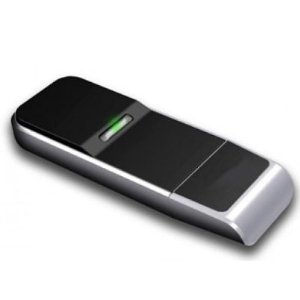
\includegraphics[width=0.2\textwidth]{./pics_comparacion_hardware/gps.jpg}
	\caption{Canmore GT-730F}
	\label{fig:gps}
\end{figure}

\newpage
\subsection{Definicin de instrumentacin}
\vspace*{15pt}


%TODO Acelermetro + girscopo Pater
En la secciones \ref{acelerometro} y \ref{giro} se detall el porqu de la eleccin de la tecnologa MEMS para el acelermetro y el girscopo. Las razones fundamentales son el costo, tamao y peso de los instrumentos, siendo los ltimos dos crticos en la aplicacin.
A partir de esta definicin surgen dos posibilidades, integrar los instrumentos diseando un PCB o adquirir uno en el cual se encuentren los dos sensores. Al disear un PCB se reduce el costo de la instrumentacin. El precio de cada chip ronda los 5 U\$S, sumado al precio de algunas resistencias, capacitores y otros materiales necesarios para la construccin del PCB (Placa de cobre, percloruro, estao, etc) hacen un total muy inferior al costo de comprar una placa ya armada (ms de 60 U\$S). Sin embargo, el proceso de diseo del PCB extiende los plazos en gran medida, se debe disear el circuito, construir y verificar su funcionamiento. El proceso mencionado tendr probablemente una duracin superior a las dos semanas, lo cual implica un retraso en varios aspectos del proyecto ya que diversas tareas previamente definidas dependen fuertemente del funcionamiento de la instrumentacin. Por otra parte el peso que representa el costo de adquirir una placa en la que se incluyan ambos sensores (acelermetro y girscopo) en el presupuesto total es muy bajo (4\%).

A partir de el anlisis realizado se decide por adquirir una placa ya diseada que contenga los sensores necesarios. Existe una gran diversidad de soluciones de instrumentacin en el mercado. Debido a los requerimientos del proyecto se descartaron muchas de ellas. Las opciones consideradas finalmente se resumen en una tabla en el anexo. La caracterstica comn a todas ellas es que pueden medir 6 grados de libertad, la misma cantidad de variables del sistema a controlar (tres coordenadas correspondientes a la posicin del centro de masa, raw, yaw, pitch) %TODO ANEXO.

Los criterios que se fijaron para definir la instrumentacin fueron los siguientes:
\begin{itemize}
\item
Rango de medidas de los sensores
\item
Capacidad de cmputo
\item
Facilidad de programacin (algunas placas incluyen microprocesadores)
\item
Comunicacin disponible 
\item
Compatibilidad con el resto del sistema
\item
Costo
\end{itemize}

En lo que respecta al rango de medida de los acelermetros se defini que el mismo fuera de 3g. Dicha eleccin est fundamentada en que se planea un vuelo en el cual no se precisen considerar aceleraciones que sean muy superiores a la de la cada libre.  Asimismo, se defini como rango de medida de los girscopos un valor  superior a los 300/s, de forma que el sistema pueda realizar un giro casi completo en cualquiera de los tres ejes en 1 segundo. 
%TODO Masmenos 3g y masomenos 300
Lo que se observa es que todos los acelermetros y giroscopos de las placas de esta preseleccin cumplen con dicho requerimiento.


\begin{table}[H]
\begin{tabular}{p{115pt}|p{55pt}|p{65pt}|p{55pt}|p{90pt}|} 
\cline{2-5} 
& \multicolumn{2}{|c|}{\cellcolor[gray]{0.7}\textbf{Acelermetro}} 
& \multicolumn{2}{|c|}{\cellcolor[gray]{0.7}\textbf{Girscopo}}  \\ \cline{2-5}
& \cellcolor[gray]{0.8} \textbf{Rango} 
& \cellcolor[gray]{0.8} \textbf{Sensibilidad}
& \cellcolor[gray]{0.8} \textbf{Rango} 
& \cellcolor[gray]{0.8} \textbf{Sensibilidad} \\ \cline{2-5} \hline
\multicolumn{1}{|c|}{\cellcolor[gray]{0.8}\textbf{CHR-6d}}
& 3g & 300mV/g &  400/s  100/s &  2.5mV/(/s)  2.5mV/(/s) \\ \hline
\multicolumn{1}{|p{115pt}|}{\cellcolor[gray]{0.8}\textbf{Atomic IMU}}
&  1.5g  ;  6g &  800mV/g   200mV/g &  300/s  &  3.3mV/(/s)\\ \hline
\multicolumn{1}{|p{115pt}|}{\cellcolor[gray]{0.8}\textbf{IMU Digital Combo Board}}
&  2g  ;  16g &  356LSB/g   321LSB/g &  2000/s  &  14.375 LSB/(/s)\\ \hline
\multicolumn{1}{|p{115pt}|}{\cellcolor[gray]{0.8}\textbf{IMU Analgo Combo Board Razor}}
&  3g &  300mV/g  &  300/s  1200/s &  3.3mV/(/s)  0.83mV/(/s)\\ \hline
\multicolumn{1}{|p{115pt}|}{\cellcolor[gray]{0.8}\textbf{IMU Fusion Board}}
&  2g &  256 LSB/g  &  250/s  2000/s &  131 LSB/(/s)     16.4 LSB/(/s)\\
\hline 
\end{tabular}
\caption{Sensores}
\label{tab:sensores}
\end{table}

Resulta conveniente que la instrumentacin posea un microprocesador, la razn es que le ahorra tiempo a la inteligencia del sistema en el procesamiento de las medidas crudas de los sensores. Los sensores presentan sus medidas constantemente en forma analgica o digtal dependiendo del sensor en cuestin. En caso de ser una medida analgica se debe en primer lugar digitalizar. Una vez que se tiene la medida digitalizada se debe realizar un procesamiento que consiste bsicamente en ponerle una marca de tiempo a cada medida y asociarle una etiqueta correspondiente al sensor que la realiz. 
%TODO ver si finalmente lo hacemos as
Resulta sumamente interesante que no sea el \emph{core} quien se encarga de esta identificacin, sino que obtenga los datos pre-procesados. Por esta razn se favorecieron las placas que incluyeran un microprocesador. 


\begin{table}[H]
\begin{tabular}{p{110pt}|p{65pt}|p{65pt}|p{60pt}|p{60pt}|} 

\cline{2-5} 
& \cellcolor[gray]{0.8} \textbf{Frecuencia reloj} 
& \cellcolor[gray]{0.8} \textbf{Largo de palabra}
& \cellcolor[gray]{0.8} \textbf{RAM} 
& \cellcolor[gray]{0.8} \textbf{Flash}\\ \cline{2-5} \hline
\multicolumn{1}{|p{110pt}|}{\cellcolor[gray]{0.8}\textbf{CHR-6d}}
&  72MHz &  32 bits &  20Kb &  64Kb \\ \hline
\multicolumn{1}{|p{110pt}|}{\cellcolor[gray]{0.8}\textbf{Atomic IMU}}
&  10MHz  &  8 bits &  2Kb  &  32Kb \\ \hline
\multicolumn{1}{|p{110pt}|}{\cellcolor[gray]{0.8}\textbf{IMU Digital Combo Board}}
&  - &  - &  -  &  -\\ \hline
\multicolumn{1}{|p{110pt}|}{\cellcolor[gray]{0.8}\textbf{IMU Analgo Combo Board Razor}}
&  - &  -  &  - &  -\\ \hline
\multicolumn{1}{|p{110pt}|}{\cellcolor[gray]{0.8}\textbf{IMU Fusion Board}}
&  - &  -  &  - &  -\\
\hline 
\end{tabular}
\caption{Caractersticas de los microprocesadores}
\label{tab:micro}
\end{table}

En caso de optar por una placa con microprocesador resulta fundamental que la misma sea sencilla de programar. Las razones son evidentes, si los algoritmos que vienen programados de fbrica no resultan adecuados para la aplicacin se pueden modificar fcilmente. Tambin parece importante que el cdigo de fbrica sea abierto; en primer lugar para comprender su funcionamiento y poder procesar adecuadamente los datos que se obtengan de los sensores. Es interesante adems poder modificar secciones puntuales de cdigo, sin necesidad de reprogramar completamente el microprocesador. 

La comunicacin no result un factor crtico ya que todos los candidatos a \emph{core} poseen diversas interfaces (UART, I2C, Converoares AD). Sin embargo, debido a la familiarizacin que se tena con las comunicaciones serie se prefiri dar prioridad a aquellas placas que se comunicaran Via UART (en caso que se optara por una placa con microprocesador).

En lo que respecta a compatibilidad con el sistema, se busc que la alimentacin de la placa sea la misma que la del microprocesador principal. Por dicha razn lo ideal es que la placa pueda ser alimentada a 5V.

A partir de las consideraciones anteriores, se considera que la solucin ms adecuada para el objetivo que se plantea en esta seccin es la placa Atomic IMU. Dicha placa cumple con los rangos de medida especificados anteriormente, posee un microprocesador de 8 bits con un reloj de 10MHz. Existe ya un cdigo en c disponible para programar el dispositivo. El mismo puede ser modificado en caso de no cumplir con todos los requerimientos necesarios. La placa dispone de un puerto JTAG para la programacin del mismo. La forma que tiene la placa de presentar los datos obtenidos de los sensores es a travs de un puerto serie capaz de transmitir datos con una tasa de transferencia de 115.200bps. Cabe aclarar que la Atomic IMU es la nica de las soluciones consideradas que puede ser alimentada con una fuente de tensin de 5V. Por otra parte el costo de la misma es de los ms bajos dentro de las posibilidades consideradas.

En la figura \ref{fig:IMU} se puede observar la instrumentacin escogida:

\begin{figure}[h!]
	\centering
	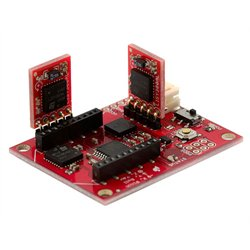
\includegraphics[width=0.3\textwidth]{./pics_comparacion_hardware/IMU.jpg}
	\caption{Atomic IMU}
	\label{fig:IMU}
\end{figure}

\end{document}

Algunos layouts para poner imgnenes. Copien y peguen noms. Hay figura comn, dos figuras en 1 onda fig 3a y 3b, wrapfigures y una matriz de figuras. Ta bueno, todas quedan lindas y andan bien.

\begin{figure}[h!]
	\centering
	\includegraphics[width=0.75\textwidth]{./Pics/		.eps}
	\caption{		}
	\label{fig:		}
\end{figure}

\begin{figure} [h!]
  \centering
  \subfloat[caption 1]{\label{fig:		}
  		\includegraphics[width=0.45\textwidth]
  			{./Pics/		.eps}}
  \subfloat[caption 2]{\label{fig:		} 
  		\includegraphics[width=0.45\textwidth]
  			{./Pics/ 		.eps}}
  \caption{Caption general}
  \label{fig:	label general	}
\end{figure}

\begin{wrapfigure}{l}{0.6\textwidth}
  \vspace{-20pt}
  \begin{center}
    \includegraphics[width=0.45\textwidth]
    	{./Pics/		.eps}
  \end{center}
  \vspace{-20pt}
  \caption{		}
  \label{ 		}
  \vspace{-10pt}
\end{wrapfigure}

\begin{figure} [h!]
  \begin{center}
    \begin{tabular}{cc}
      \resizebox{50mm}{!}
      	{\includegraphics{./Pics/ 	.eps}} &
      \resizebox{50mm}{!}
      	{\includegraphics{./Pics/	.eps}} \\
      \resizebox{50mm}{!}
      	{\includegraphics{./Pics/	.eps}} &
      \resizebox{50mm}{!}
      	{\includegraphics{./Pics/	.eps}} \\
    \end{tabular}
    \caption{ 		}
    \label{ 		}
  \end{center}
\end{figure}